
% This is based on LLNCS.dem the demonstration file of
% the LaTeX macro package from Springer-Verlag
% for Lecture Notes in Computer Science,
% version 2.4 for LaTeX2e as of 16. April 2010
%
% Modified by Gabriele Bleser, January 2013
% Modified by Oliver Wasenmüller, March 2016
% Modified by Oliver Wasenmüller, November 2017
%
% This is the Latex main document. If you need additional packages,
% you can insert them here. Otherwise, you should not modify this.
% Provide your contribution in a separate file, such as mypaper.tex.
% All contributions will be included here.
%

\documentclass{llncs}

% Include your packages here
\usepackage{graphicx}
\usepackage{textcomp}
\usepackage{listings}
\usepackage{subfiles}
\usepackage{subfigure}
\usepackage{amsmath}
\usepackage{url}
\usepackage{multirow}

\usepackage{caption}
\usepackage{cite}
\usepackage{copyrightbox}
\usepackage[bookmarksnumbered=true]{hyperref}
\hypersetup{
	colorlinks = true,
	linkcolor = red,
	citecolor = green,
	filecolor = red,
	urlcolor = blue
}

% use this for review submission only. Please comment it for final submission
\usepackage{lineno}
\linenumbers
%

\begin{document}
	
	\pagestyle{headings} % switches on printing of running heads
	
	%
	\title{Survey on Face Tracking with Deep Learning}
	%
	\titlerunning{short title} % abbreviated title (for running head)
	%
	\author{Vinay Balasubramanian\inst{1} \and Jilliam Diaz Barros\inst{2}}
	%
	\authorrunning{Your name et al.} % abbreviated author list (for running head)
	%
	\institute{\email{v\_balasubr18@cs.uni-kl.de}
		\and
		\email{jilliam\_maria.diaz\_barros@dfki.de}}
	
	\maketitle % typeset the title of the contribution
	
	\begin{abstract}
		Face tracking is the underlying task for many applications such as face recognition, expression analysis and 3D face modeling. Detecting facial landmarks in wild(unconstrained) conditions still remains a challenging task. In this paper, we review different face tracking architectures and their performance in challenging conditions. We focus on deep-learning based methods that exploit the temporal information across frames, i.e video-based methods. Recent developments include using an encoder-decoder network, recurrent network, deep reinforcement learning, and two-stream network. This paper aims to compare those approaches in terms of accuracy, the dataset(s) used for training, evaluation metrics and robustness to large head poses and occlusions.
		\keywords{Face tracking, Facial landmarks, Deep Learning, Reinforcement Learning, Temporal information}
	\end{abstract}
	
	% This is your content. Name the sections appropriately
	\section{Introduction}
	Face tracking is a computer vision task of tracking the face across all frames of a video. It can be done by tracking a bounding box around the face across frames. Another way is to track specific landmarks around the face.  Facial landmarks are localized around facial components such as eyes, ears, nose, mouth and jawline.
	Face tracking technology plays an important role in computer vision applications such as \textit{Face recognition}\cite{face_recognition}, \textit{Expression recognition}\cite{expression_recognition} and \textit{Face modeling}\cite{face_modeling}. This is a challenging problem as the videos are usually captured in unconstrained conditions. They may have illumination inconsistencies, large head poses, blurriness, occlusions, etc.
	
	There are various approaches to this problem. Some of them are image-based methods, where the models are trained on still frames and the detection also happens independently at each frame. Other methods are video-based and use an incremental-learning technique to exploit the temporal connection between successive frames. Figure \ref{generic_video_based} shows a generic high-level architecture of a video-based landmark detection pipeline. The main idea is that the frames of the video are given in a sequential manner to the model and the temporal connection between the frames is utilized to track facial landmarks.
	
	The rest of this paper is organized as follows: Section 2 lists publicly available datasets for face tracking. Section 3 presents some of the state-of-the-art face tracking approaches that use deep learning. In section 4 we compare these approaches. Section 5 concludes our paper.
	
	\begin{figure}[h!]
		\centering
		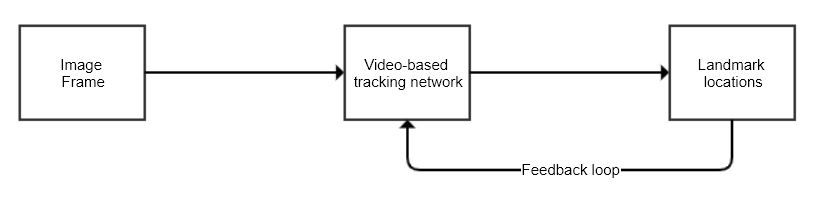
\includegraphics[scale=0.5]{Media/generic_video_based}
		\vspace{-3mm}
		\caption{Generic architecture of video based methods. Landmarks detected in the current frame are used as an initialization for the next frame}
		\label{generic_video_based}
		\vspace{-3mm}
	\end{figure}
	
	\section{Datasets}
	
	In this section, we list the datasets commonly used for landmark-based face tracking. These datasets are publicly available for research purposes. Datasets can be categorized into constrained datasets and unconstrained datasets (in the wild).
	Table \ref{datasets} shows various image-based and video datasets. Most methods use the 300-VW(300 face Videos in the Wild)\cite{300-VW} and the TF(Talking Faces)\cite{tf} datasets to evaluate their models and compete in the 300-VW challenge.
	
	%\begin{table}[]
	%\tiny
	%\centering
	%\caption{Datasets used for facial landmark detection and tracking}
	%\begin{tabular}{|l|l|l|l|l|}
	%\hline
	%\textbf{Dataset} & \textbf{Description} & \textbf{\begin{tabular}[c]{@{}l@{}}Video/\\ Image\end{tabular}} & \textbf{Contains} & \textbf{Wild?} \\ \hline
	%AFLW\cite{aflw} & \begin{tabular}[c]{@{}l@{}}Annotated Facial Landmarks \\ in the Wild\end{tabular} & Image & \begin{tabular}[c]{@{}l@{}}Around 25k annotated face images with \\ 21 landmarks per image\end{tabular} & Yes \\ \hline
	%COFW\cite{cofw} & \begin{tabular}[c]{@{}l@{}}Caltech Occluded Faces in \\ the Wild\end{tabular} & Image & \begin{tabular}[c]{@{}l@{}}1007 occluded face images with 29 \\ manually annotated landmarks\end{tabular} & Yes \\ \hline
	%Helen\cite{helen} & Helen facial feature dataset & Image & \begin{tabular}[c]{@{}l@{}}2000 training and 330 test images with \\ 194 landmarks and accurate annotations \\ of primary facial components\end{tabular} & Yes \\ \hline
	%IBUG\cite{ibug} & IBUG dataset & Image & \begin{tabular}[c]{@{}l@{}}135 images with difficult poses and \\ expressions\end{tabular} & Yes \\ \hline
	%LFPW\cite{lfpw} & Labeled Face Parts in the Wild & Image & \begin{tabular}[c]{@{}l@{}}1432 images with 29 landmarks on \\ each image\end{tabular} & Yes \\ \hline
	%LFW\cite{lfw} & Labeled Faces in the Wild & Image & \begin{tabular}[c]{@{}l@{}}13,233 images of 5749 people detected \\ and centered by Viola Jones face detector\end{tabular} & Yes \\ \hline
	%3D Menpo\cite{3d_menpo} & The 3D Menpo database & Image & \begin{tabular}[c]{@{}l@{}}14000 static images with 2D and 3D \\ landmarks and around 280,000 \\ annotated frames\end{tabular} & Yes \\ \hline
	%BIWI\cite{biwi} & Biwi kinect head pose database & Video & \begin{tabular}[c]{@{}l@{}}24 videos with over 15k frames of \\ 20 people\end{tabular} & Yes \\ \hline
	%FM\cite{fm} & Face Movies & Video & \begin{tabular}[c]{@{}l@{}}2150 images of 6 videos with 68 landmarks \\ on each image\end{tabular} & Yes \\ \hline
	%RWMB\cite{fab} & Real-World Motion Blur & Video & \begin{tabular}[c]{@{}l@{}}10000 face videos with 98 landmarks \\ including occlusion, blur, illumination \\ changes etc.\end{tabular} & Yes \\ \hline
	%SynHead\cite{dynamic_facial_analysis} & Synthetic dataset & Video & \begin{tabular}[c]{@{}l@{}}510,960 frames of 70 head motion tracks \\ that include large face pose variations\end{tabular} & Yes \\ \hline
	%TF\cite{tf} & Talking Face & Video & \begin{tabular}[c]{@{}l@{}}5000 frames of a person engaged in a \\ conversation with 68 landmarks in each \\ frame on each image\end{tabular} & No \\ \hline
	%300VW\cite{300-VW}, & 300 videos in the wild & Video & \begin{tabular}[c]{@{}l@{}}114 videos with 218,595 frames with \\ 68 landmarks per frame\end{tabular} & Yes \\ \hline
	%\end{tabular}
	%\label{datasets}
	%\end{table}
	\vspace{-8mm}
	\begin{table}[]
		%\tiny
		\begin{center}%\centering
			\caption{Datasets used for facial landmark detection and tracking}
			\begin{tabular}{|l|l|c|l|c|c|}
				\hline
				\multirow{2}{*}{\textbf{Dataset}} & \multirow{2}{*}{\textbf{Description}} & \textbf{Video/} & \multirow{2}{*}{\textbf{Contains}} & \multirow{2}{*}{\textbf{Points}} & \multirow{2}{*}{\textbf{Wild}} \\
				& & \textbf{Image} & & & \\
				\hline
				
				\multirow{2}{*}{AFLW\cite{aflw}} & Annotated Facial Landmarks & \multirow{2}{*}{Image} & \multirow{2}{*}{Around 25k annotated face images.} & \multirow{2}{*}{21} & \multirow{2}{*}{Yes} \\
				& in the Wild & & & & \\
				\hline
				
				\multirow{2}{*}{COFW\cite{cofw}} & Caltech Occluded Faces & \multirow{2}{*}{Image} & \multirow{2}{*}{1007 occluded face images.} & \multirow{2}{*}{29} & \multirow{2}{*}{Yes} \\
				& in the Wild & & & & \\
				\hline
				
				\multirow{2}{*}{HELEN\cite{helen}} & HELEN facial feature & \multirow{2}{*}{Image} & 2000 training and 330 test images. & \multirow{2}{*}{194} & \multirow{2}{*}{Yes} \\
				& dataset & & Includes additional annotations. & & \\
				\hline
				
				\multirow{2}{*}{IBUG\cite{ibug}} & \multirow{2}{*}{IBUG dataset} & \multirow{2}{*}{Image} & 135 images with difficult poses & \multirow{2}{*}{68} & \multirow{2}{*}{Yes} \\
				& & & and expressions. & & \\
				\hline
				
				LFPW\cite{lfpw} & Labeled Face Parts in the Wild & Image & 1432 images. & 29 & Yes \\
				\hline
				
				LFW\cite{lfw} & Labeled Faces in the Wild & Image & 13,233 images of 5749 people. & 10 & Yes \\
				% & & & centered by Viola Jones face detector. & \\
				\hline
				
				3D Menpo & \multirow{2}{*}{The 3D Menpo database} & Image & Around 12k images and 280k video & \multirow{2}{*}{84} & \multirow{2}{*}{Yes} \\
				\cite{3d_menpo} & & \& Video & frames, with 2D and 3D landmarks. & & \\
				\hline
				
				300-W\cite{300-W} & 300 Faces-In-The-Wild & Image & 600 images in the wild & 68 & Yes \\
				% & & & centered by Viola Jones face detector. & \\
				\hline
				
				FM\cite{fm} & Face Movies & Video & 2150 images of 6 videos. & 68 & Yes \\
				\hline
				
				RWMB\cite{fab} & Real-World Motion Blur & Video & 20 videos with motion blur. & 68/98 & Yes \\
				\hline
				
				\multirow{2}{*}{TF\cite{tf}} & \multirow{2}{*}{Talking Face} & \multirow{2}{*}{Video} & 5000 frames of a person engaged & \multirow{2}{*}{68} & \multirow{2}{*}{No} \\
				& & & in a conversation. & & \\
				\hline
				
				300VW\cite{300-VW} & 300 videos in the wild & Video & 114 videos with 218,595 frames. & 68 & Yes \\
				\hline
			\end{tabular}
			\label{datasets}
		\end{center}
	\end{table}
	\vspace{-13mm}
	\section{Face Tracking Approaches}
	In this section, we describe some of the state-of-the-art approaches for video-based facial landmark tracking. Deep learning methods, in general, use CNN and RNN to detect landmarks.
	
	\subsection{Dynamic Facial Analysis using Recurrent Neural Networks (2017) \cite{dynamic_facial_analysis}}
This approach uses RNN for head pose estimation and facial landmark tracking.
It proposes RNN as an alternative approach that performs better than previous video-based approaches for dynamic facial analysis which use Kalman filters or particle filters. The method is inspired by the fact that RNNs and Bayesian filters are operationally very similar, although Bayesian filters need problem-specific hand-tuning. Given sufficient data, an RNN can be trained to do the same task and avoid problem-specific tracker engineering.
The authors create a synthetic dataset \textbf{SynHead} to cater to the need for large training data.

The approach employs FC-RNN to exploit the generalization from a pre-trained CNN and consists of CNN layers followed by recurrent layers as dense layers. Figure \ref{cnn_rnn} shows the proposed architecture for head pose estimation and tracking. The CNN and RNN are trained together end-to-end. The head pose is estimated in terms of pitch, yaw and roll angles. The network is a modified VGG16 with an extra fully connected layer with 1024 neurons and the output layer consists of 3 neurons for the pitch, yaw and roll angles. For facial landmark detection, the same network is used with the only difference that the output layer contains 136 neurons corresponding to the locations of the 68 landmarks. RNN makes the model robust to occlusions and large head poses.
The weights of the RNN are fixed once the training is complete, and the model cannot adapt dynamically to new data.

\begin{figure}
	\centering
	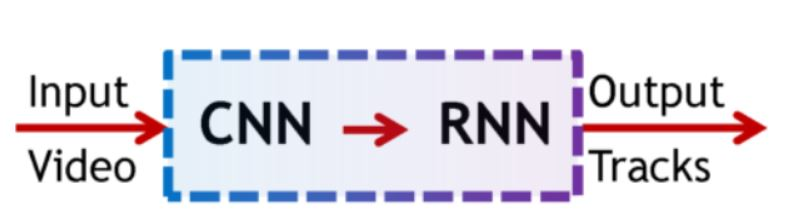
\includegraphics[scale=0.3]{Media/cnn_rnn}
	\vspace{-3mm}
	\caption{Proposed end-to-end CNN RNN network. Source:\cite{dynamic_facial_analysis}}
	\label{cnn_rnn}
	\vspace{-3mm}
\end{figure}

	\subsection{Two Stream Transformer Networks (2017) \cite{tstn}}
This approach proposes a two-stream deep learning method that decomposes the video input to spatial and temporal streams. The spatial stream aims to capture appearance information from still frames and it is trained to transform image pixels to landmark positions directly on still frames and then to refine the current facial shape based on the previous shape. On the other hand, the temporal stream aims to capture temporal consistency information across successive frames.

Figure \ref{TSTN} shows the proposed TSTN architecture. The temporal stream consists of an encoder-decoder module. The encoder is trained to encode the spatial information as active appearance codes that capture the whole face changes across frames in the temporal dimension. The decoder remaps the learned codes to the original face input size. The temporal consistency information for each landmark is used to improve alignment accuracy. It also consists of a two-layer RNN in between the encoder-decoder module. The first layer captures spatial-temporal appearance features whereas the second layer memorizes the temporal information across frames. Facial landmarks are determined by a weighted fusion of both spatial and temporal streams. The landmark positions are refined simultaneously in both the streams.
The weights for the fusion of both the streams are not learnable and has to be set manually. The authors conducted experiments for different weights{(100,0), (0,100), (80,20), (20,80), (50,50)} and achieved the best performance for equal weight of 50\% for both the streams
\begin{figure}
	\centering
	\vspace{-7mm}
	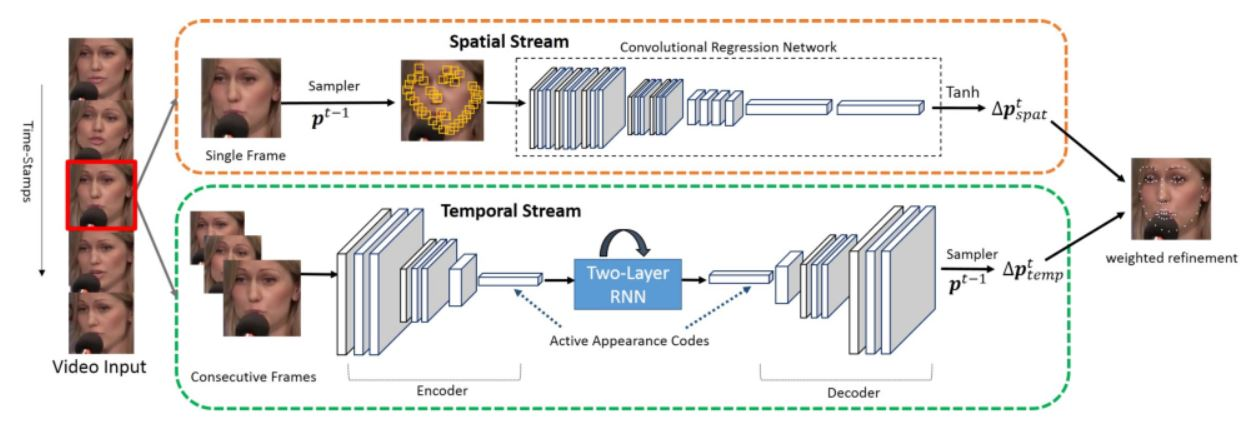
\includegraphics[scale=0.5]{Media/TSTN}
	\vspace{-3mm}
	\caption{TSTN pipeline. Source:\cite{tstn}}
	\label{TSTN}
	\vspace{-3mm}
\end{figure}
\vspace{-8mm}
	\subsection{Face Alignment Recurrent Network (2017) \cite{farn}}

Previous state-of-the-art regression-based approaches start with an initial shape estimation and iteratively estimate the facial shape at successive stages by estimating an increment from the previous estimation. This paper proposes to improve the cascade shape regression by using LSTM and Region Convolutional Neural Network (RCNN). The LSTM model exploits both spatial and temporal information for landmark detection in images and videos in uncontrolled conditions. The predicted landmark location is used as a basis for estimation in the next stage and frame in spatial and temporal dimensions. The process continues recurrently until the face shape is finalized. The proposed model is for facial landmark detection in images under uncontrolled conditions and not for facial landmark tracking.

Figure \ref{farn_training} shows the training architecture of Face Alignment Recurrent Network(FARN). The face image, initial face shape, and ground truth shape are given as input to the network. The image is passed through several convolutional and max-pooling layers to obtain a feature map. The initial face shape contains facial landmarks. Region of Interest (ROI) pooling is applied around each landmark to obtain ROI pooling features. The ROI pooling features are concatenated and given to a fully connected layer followed by an LSTM layer. The network outputs the predicted shape increment over the initial face shape. The initial face shape is summed over the predicted shape increment to obtain updated initial face shape. This process continues recurrently for $T$ stages.

\begin{figure}
	\centering
	\vspace{-5mm}
	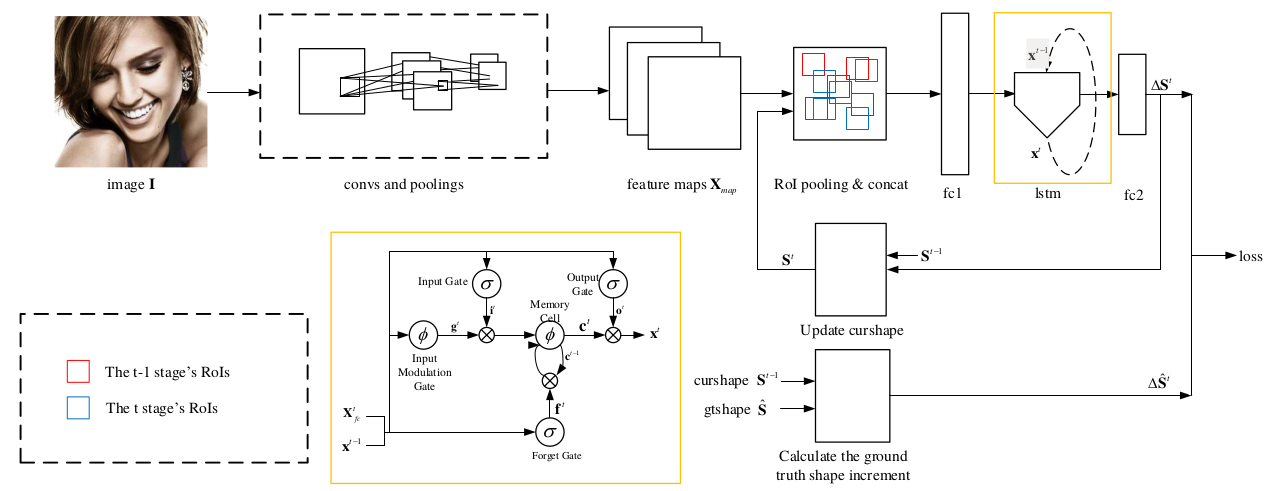
\includegraphics[scale=0.3]{Media/farn_training2}
%	\vspace{-3mm}
	\caption{FARN training architecture. Source:\cite{farn}}
	\label{farn_training}
	\vspace{-10mm}
\end{figure}
\vspace{-1mm}
	\subsection{Recurrent Encoder-Decoder Network for Video-based Face Alignment (2018) \cite{rednet}}
	This method leverages temporal information to predict facial landmarks in each frame and uses recurrent learning at both spatial and temporal dimensions. At the temporal level, the features are separated into \textit{temporal-variant} features such as pose and expression, and \textit{temporal-invariant} features such as facial identity. Recurrent learning is only applied to the temporal-variant features. This feature disentangling has shown to achieve better generalization and more accurate results. Figure \ref{rednet_architecture} shows the pipeline of recurrent encoder-decoder network (REDNet).
	
	\begin{figure}
		\centering
		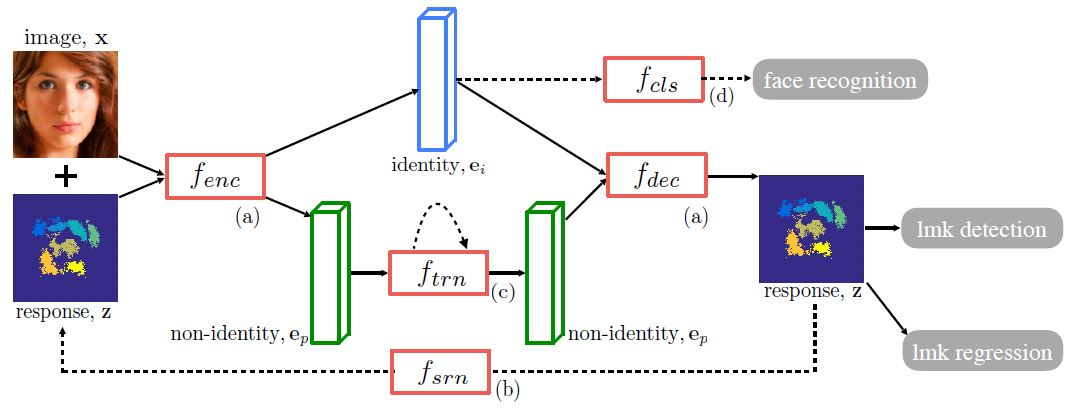
\includegraphics[scale=0.5]{Media/rednet_architecture}
		\vspace{-3mm}
		\caption{Overview of REDNet pipeline. Source:\cite{rednet}}
		\label{rednet_architecture}
		\vspace{-3mm}
	\end{figure}
	%\vspace{-1mm}
	
	The network consists of 4 modules:
	\begin{itemize}
		\item[(1)] \textbf{Encoder-Decoder}:-
		The encoder encodes features from a single video frame into an intermediate low dimensional representation by performing a sequence of convolutions, pooling and batch normalization. The decoder upsamples the low dimensional representation and transforms it into a response map that contains facial landmarks.
		\item[(2)] \textbf{Spatial recurrent learning}:-
		The purpose is to find the exact location of landmarks in a coarse-to-fine manner by iteratively providing the previous prediction as feedback along with the video frame. This is carried out in 2 steps - \textit{Landmark Detection} and \textit{Landmark Regression}. Landmark detection step locates 7 major facial components whereas landmark regression step refines predicted locations of all 68 landmark positions
		\item[(3)] \textbf{Temporal recurrent learning}:-
		This is proposed to model the temporal-variant factors such as pose and expression. The temporal variations in the temporal-invariant factors (non-identity code) are modeled using a Long Short Term Memory(LSTM) unit consisting of 256 hidden neurons.
		Trained using \textit{T} successive frames. Detection and regression tasks are performed frame by frame.
		\item[(4)] \textbf{Supervised identity disentangling}:-
		Complete identity and non-identity factor disentangling cannot be guaranteed. More supervised information is needed to achieve better separation of the features. This module applies identity constraint to the identity code(temporal-invariant factors) to further separate identity code from the non-identity code(temporal-variant factors). Face recognition is applied to the identity code to classify the people present in the frames. This is shown to yield better generalization and better test accuracy\\
	\end{itemize}
	This model may have high computational complexity due to the spatial recurrent learning block and the usage of VGG16 for the encoder and the decoder.
	



	\subsection{Dual-Agent Deep Reinforcement Learning (2018) \cite{dadrl}}
	This approach exploits the fact that bounding box tracking and landmark detection are dependent. The accuracy of the detected facial landmarks depends on how good the bounding box is.
	Figure \ref{deformable_face_tracking} shows different strategies for deformable face tracking including the proposed DADRL (Dual-Agent Deep Learning) architecture. This framework is designed for simultaneous bounding box tracking and landmark detection in an interactive manner and uses reinforcement learning to learn to make adaptive decisions during face tracking. The architecture consists of a \textit{Tracking agent}, an \textit{Alignment agent} and \textit{communication channels} between the agents, as shown in Figure \ref{dadrl_architecture}. The two agents are trained simultaneously to learn two conditional distributions. The message channels are trained using deep Q-learning algorithm.
	
	\begin{figure}
		\centering
		\vspace{-7mm}
		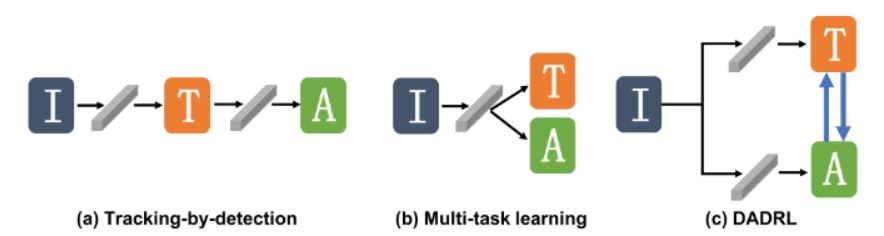
\includegraphics[scale=0.5]{Media/deformable_face_tracking}
		\vspace{-3mm}
		\caption{Strategies for deformable face tracking. Source:\cite{dadrl}}
		\label{deformable_face_tracking}
		\vspace{-3mm}
	\end{figure}
	\vspace{-1mm}
	\begin{figure}
		\centering
		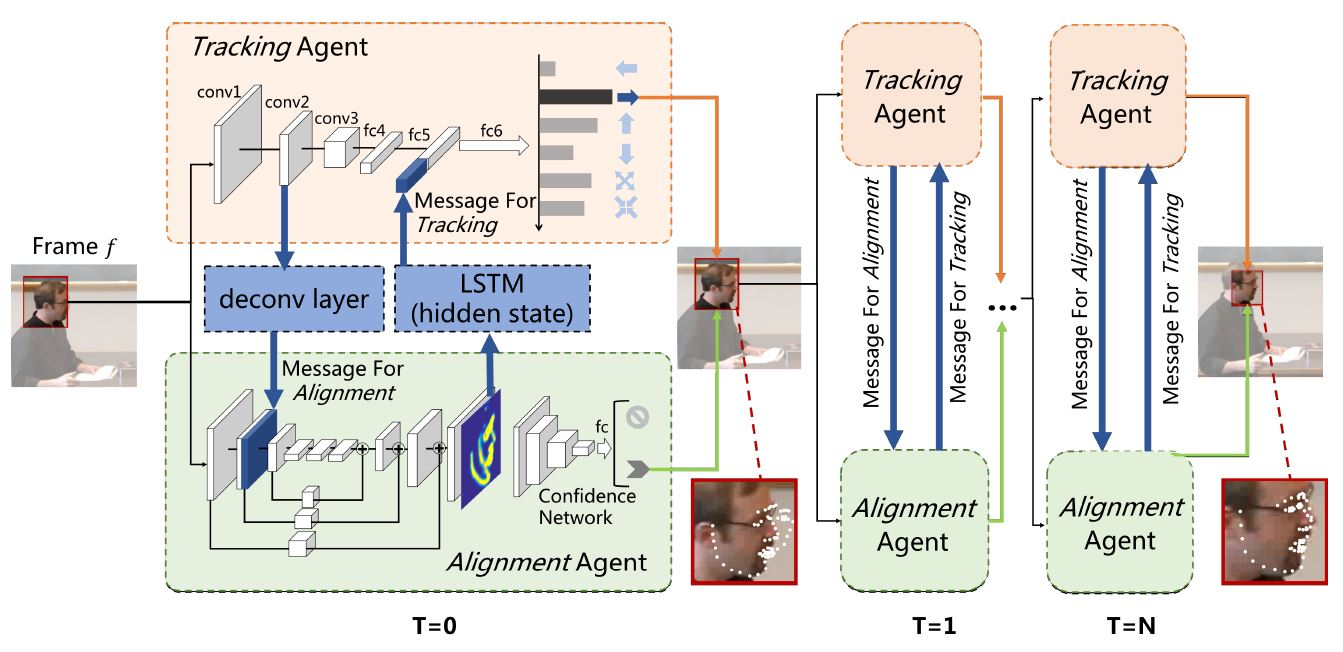
\includegraphics[scale=0.5]{Media/DADRL}
		\vspace{-3mm}
		\caption{DADRL architecture. Source:\cite{dadrl}}
		\label{dadrl_architecture}
		\vspace{-3mm}
	\end{figure}
	\vspace{-1mm}
	If $I_k$ is the $k^{th}$ frame, $B_k$ is the bounding box for the $k^{th}$ frame and $V_k$ is the vector of $L$ landmarks, then the probabilistic duality is given by:
	
	\begin{equation}
	p\left(B_{k} | I_{k}\right) p\left(V_{k} | B_{k}, I_{k}\right)=p\left(V_{k} | I_{k}\right) p\left(B_{k} | V_{k}, I_{k}\right)
	\end{equation}
	
	The learning objectives of bounding box tracking and landmark detection are treated as two conditional probabilities and the dependency between these two tasks is formulated as two marginal distributions. Since the ground-truth marginal distributions are not available, communication channels between the agents are used as alternatives to satisfy the probabilistic duality. For each frame, the terminal state of the previous frame is used for initializing the current state. The two agents decide a sequence of actions based on the observed state and exchanged messages, to adjust the bounding box and regress facial landmarks simultaneously. The messages sent from the tracking agent to the alignment agent are encoded by a deconvolution layer. It provides additional textural information to the alignment agent to improve its robustness. The messages from the alignment agent to the tracking agent are encoded by an LSTM unit. It provides 3D pose information to the tracking agent to improve bounding box tracking.
	

	\vspace{-5mm}
	\section{Performance Comparison}
	In this section we compare the above methods starting from the datasets used for training and testing, evaluation metrics, evaluation on common dataset and robustness to challenges.
	
	\textbf{Dynamic Facial Analysis} \cite{dynamic_facial_analysis} is trained using the created SynHead dataset with the L2 loss function and tested on the BIWI dataset for head-pose estimation. It is then fine-tuned using training data from the BIWI dataset. For landmark detection, the corresponding model is trained and tested using a randomly split 300-VW dataset. For each frame, the mean Euclidean distance of the 68 landmarks is computed. It is normalized by the diagonal distance of the ground truth box. The metrics used for evaluation are \textit{area under the curve}(AUC) and \textit{failure rate}(FR). AUC is the area under the cumulative error distribution curve. FR is the percentage of images whose errors are larger than a given threshold. The proposed RNN-based architecture is more robust to large head poses and occlusions compared to per-frame estimation.
	
	\textbf{TSTN} \cite{tstn} is trained using the 300-VW training set. The pre-trained spatial stream network is finetuned beforehand. The model is evaluated on the testing sets of Talking Face(TF) and 300-VW datasets. Normalized Root-Mean-Square-Error and cumulative error distribution plots are used for evaluating the model. The temporal stream consisting of the encoder-decoder module and the 2-layer RNN provides consistency over time.  The spatial stream which provides complementary appearance information from still frames, achieves robustness to large head poses, occlusions and variations of expressions.
	
	\textbf{FARN} \cite{farn} is trained on the training partition consisting of training sets of COFW, LFPW, Helen and the entire AFW with 3148 images in total. The testing partition contains 3 parts - the common subset, the challenging subset, and the full set. The common subset consists of testing set of LFPW and Helen with 554 images in total. The challenging subset consists of the IBUG dataset which contains additional annotations for 135 images in difficult poses and expressions. The full set consists of both the common subset and the challenging subset with 689 images. The model is evaluated using point-to-point Root-Mean-Square-Error between the face shape and the ground truth annotations. The end-to-end trained model runs extremely fast (18ms) with robustness to large head poses and occlusions.
	
	\textbf{REDNet} \cite{rednet} is trained on both image and video datasets with different configurations for different datasets. The training happens in 3 steps. In the first step, the network without the temporal recurrent learning and supervised identity disentangling modules is pre-trained using the image datasets AFLW, Helen and LFPW. In the second step, supervised identity disentangling is included and trained with other modules using the image-based LFW dataset. In the third step, the temporal recurrent learning module is included and the entire model is fine-tuned using the video dataset 300-VW. Inter-ocular distance is used to normalize the Root-Mean-Square-Error(RMSE).
	The coarse-to-fine strategy in the two-step spatial recurrent learning(landmark detection and landmark regression) makes the model robust to large head pose and partial occlusions.
	
	\textbf{DADRL} \cite{dadrl} is trained in two stages. The \textbf{first stage} is the \textit{supervised learning stage} in which the two agents are trained separately. All training data from 300 faces in the wild challenge (300-W image dataset) is used to train the alignment agent. The 300-VW training set is used to train the tracking agent. The communicated messages are set to zero in this stage. The \textbf{second stage} is the \textit{reinforcement learning stage} in which the whole network is trained with the 300-VW training set. The model is evaluated on the test set of 300-VW. For evaluation, Normalized Root-Mean-Square-Error and cumulative error distribution plots are used. The communication channels between the agents has shown to provide robustness to occlusions. The authors also propose a DADRL-3D which is trained on the 3D Menpo dataset \cite{3d_menpo}. It is more robust to large pose as it is trained on 3D data.
	

	
	REDNet\cite{rednet}, Dynamic Facial Analysis\cite{dynamic_facial_analysis}, TSTN\cite{tstn} and FARN\cite{farn} provide testing results on challenging category of 300-VW test set for 68 landmarks. REDNet\cite{rednet} and TSTN\cite{tstn}(7 landmarks) provide results on Talking Face dataset \cite{tf}. REDNet\cite{rednet} provides results for both 68 and 7 landmarks in both datasets.
	Table \ref{comparison} reports the RMSE of the compared methods on 300-VW and TF\cite{tf} datasets.
	DADRL\cite{dadrl} reports normalized RMSE for a few videos with heavy occlusions from the most challenging Category 3 of 300-VW. It has the lowest error among the others on the 300-VW dataset for 68 landmarks.
	REDNet\cite{rednet} reports RMSE for Category 3 of 300-VW dataset and TF dataset for both 7 and 68 landmarks. TSTN\cite{tstn} shows the best performance on the controlled TF dataset for 7 landmarks. Although FARN\cite{farn} does not have the lowest error, it performs in real time (18ms). DADRL-3D is the only method that tracks 3D landmarks.
	
	\vspace{-8mm}
	\begin{table}[]
		\centering
		\caption{Evaluation on 300-VW and TF test sets}
		\begin{tabular}{|l|c|c|c|c|}
			\hline
			& \multicolumn{2}{c|}{\textbf{300-VW}} & \multicolumn{2}{c|}{\textbf{TF}} \\ \hline
			\textbf{Method} & \textbf{\begin{tabular}[c]{@{}l@{}}RMSE(68 \\ landmarks)\end{tabular}} & \textbf{\begin{tabular}[c]{@{}l@{}}RMSE(7 \\ landmarks)\end{tabular}} & \textbf{\begin{tabular}[c]{@{}l@{}}RMSE(68 \\ landmarks)\end{tabular}} & \textbf{\begin{tabular}[c]{@{}l@{}}RMSE(7 \\ landmarks)\end{tabular}} \\ \hline
			Dynamic Facial Analysis\cite{dynamic_facial_analysis} & 6.16 & - & - & - \\ \hline
			TSTN\cite{tstn} & 5.59 & - & - & \textbf{2.13} \\ \hline
			FARN\cite{farn} & 5.90 & - & - & - \\ \hline
			REDNet\cite{rednet} & 5.15 & \textbf{5.29} & \textbf{2.77 } & 2.89 \\ \hline
			
			DADRL\cite{dadrl} & \textbf{3.09} & - & - & - \\ \hline

		\end{tabular}
		\label{comparison}
	\end{table}
	\vspace{-8mm}
	

	\section{Conclusion}
	
	In this paper, we have reviewed some of the state-of-the-art deep learning methods for video-based face alignment. All of these methods avoid hand-engineering by using neural networks. All these methods use RNN in common to model temporal information. Dynamic facial analysis\cite{dynamic_facial_analysis} uses CNN followed by RNN to exploit temporal information. TSTN\cite{tstn} uses spatial and temporal streams to capture appearance information on still frames and temporal information across frames. FARN\cite{farn} uses LSTM to detect facial landmarks. REDNet\cite{rednet} uses an encoder-decoder network to separate temporal-variant and temporal-invariant factors and applies recurrent learning to the temporal-variant factors. DADRL \cite{dadrl} exploits the dependency between bounding box generation and facial landmark tracking by treating the two tasks as agents and using deep Q-learning to maximize the accuracy in facial landmarks over several iterations. Although the recent methods have shown robustness to large head poses and occlusions, face tracking under difficult illumination is still a challenge.
	
	\vspace{-3mm}
	
	%
	
	%
	% ---- Bibliography ----
	%
	\bibliographystyle{plain}
	\bibliography{bibexample}
	%
\end{document}